\documentclass[12pt, titlepage]{article}

\usepackage{fullpage} %full page typesetting
\usepackage{setspace} %allows for non-singlespacing
\usepackage{graphicx} %graphics capabilities
\usepackage{latexsym} %extra symbols
\usepackage{rotating} %rotation for figures
\usepackage{longtable} %tables that fill more than a single page
%\usepackage{hyperref} %hypertext links in the document
\usepackage{natbib} %better bibliographies
\usepackage{authblk} %author and affiliation in opening
\usepackage{mathpazo} %use palatino font, rather than times
\usepackage{appendix}
\usepackage{lscape}
\usepackage{tabulary}
\usepackage[nottoc]{tocbibind}
\usepackage[colorlinks=true,linkcolor=blue,citecolor=cyan]{hyperref}
\usepackage{ifthen}
\usepackage{float}

\title{\tb{Place of Residence and Political Attitudes in Democracies Worldwide }}

\author{Jennifer Lin}
\affil{New College of Florida}

\newcommand\e{\emph}
\newcommand\tb{\textbf}
\newcommand\un{\underline}
\newcommand\txt{\texttt}

\doublespacing 

\begin{document}

\begin{singlespace}
\maketitle
\end{singlespace}

\begin{center} %center text
\section*{Abstract} %the star stops this section from appearing in the ToC
	
\begin{quote}
After the 2016 election, many major new pundits pointed at Rural America as the major source of Donald Trump’s victory for the presidency. This is because, as prior research by \cite{walsh_putting_2012} for the United States and \cite{walks_city-suburban_2005} for Canada suggests, residents in rural parts of democratic countries tend to be more religious and less exposed to diversity as their urban counterparts. As a result, they are more conservative in their social views even if they may be more liberal on their fiscal ones. President Trump took advantage of this and won the hearts and minds of many voters in the Midwest and Rural South, which allowed him to secure an electoral college victory despite falling short on the popular vote. For this research project, I was interested to see if this trend extends to other developing and consolidated democracies in the world. Using the CSES Module IV data (2011-2016), I conducted regressions to test place of residence on a self-defined ideological scale and an objective ideology scale constructed using respondent opinions on various issues. By controlling for regime factors such as age and level of democracy, I find statistical significance to suggest that place matters. The data provides sufficient evidence to suggest that if one lives in an urban place compared to a rural one, they are more likely to self-identify as more liberal and hold those values when voicing their opinions on social issues.

\end{quote}
\end{center}

\clearpage

\tableofcontents
%\addcontentsline{toc}{section}{\listfigurename}
%\addcontentsline{toc}{section}{\listtablename}
\clearpage

\listoftables
\clearpage

\listoffigures
\clearpage

\section{Introduction}

After the election of Donald Trump as the 45th President of the United States, news pundits speculate that the reason for his election was through the support that he won from rural voters in the South and Midwest. These Republican strongholds located in the rural and suburban parts of the country have been researched by political scientists \citep{walsh_putting_2012} and the results suggest that there is an urban-rural divide that is growing in the United States. Additionally, it is noticeable that the mindset of individuals who live in different parts of the country do not conceptualize politics in a similar fashion \citep{holloway_burning_2007}. These differences in interests leads to differences in ideologies and attitudes, as seen in the United States back in 2016.

However, the United States does not operate in isolation and the people are not necessarily idiosyncratic compared to others around the world. Therefore, in this paper, I am interested in understanding if the urban-rural divide that is present in the US is also present and noticeable in other places around the globe. Additionally, I  will discuss how living in a different environment leads people to favor different interests and hold distinct political beliefs in the context of key regime factors such as the level of democracy, age of regime and the type of electoral formula that a regime employs in their system of government.
 
Through the analysis of the Comparative Study of Electoral Systems (CSES) Module IV data, I find that place of residence does matter in influencing one's political beliefs and ideologies. More specifically, the results will allow us to draw two conclusions. First, the place of residence matters in influencing political attitudes, but this is heavily influenced on the regime's electoral formula such that if a respondent lives in a first past the post system, there is a greater pronounced difference between place of residence and ideology, but this effect is not significant in proportional representation systems. Second, the influence of place of residence on political ideology is more pronounced in more established and longstanding democracies than developing ones such that the divide between urban, suburban, small town, and rural residents are more pronounced when the regime has a system of democracy that has been instituted for a longer period of time.
 
\section{Theoretical Review of Literature}

Past research in this topical area considered the influence of place in specific case studies. These results will be analyzed in this section of the paper, followed by an analysis of general conclusions that these cases suggest. I will also briefly introduce the countries that are being included in this paper and conclude the section with a word of caution before moving to the data analysis. 

\subsection{Trends of Urban-Rural Divide in Seen in Previous Case Studies}

The most popular places where literature exists for understanding the urban-rural divide in political attitudes lies mostly in the developed world. Namely, the United States, and Canada are the top countries where this trend has been analyzed most frequently. As we will see later, these are also the two countries that do not have the full supply of data in the Comparative Study of Electoral Systems data to be included in this paper. Therefore, I will consider the lessons learned from these two places, along with some others, as a way to gain some insight on the extent of rural-urban influence on political attitude development in a developed democracy in hopes of understanding how other polities differ in their own unique ways to the conditions of the polity.

\subsubsection{The United States}

\subsubsection{Canada}

\subsubsection{Other Countries}

In the general light, residents in one area often view a neighboring, unfamiliar region by the seterotypes that define it. In France, this is quite the case \citep{clout_new_2003}. Urban residents see the rural plains as undeveloped lands that are waiting for thier entrepreneurial talents. Yet, rural interests often go unnoticed unless a party that would speak for them is in power. Yet, the people of France, on all sides of the picture, are not alone. In this section, I will consider other countries where signs of an urban-rural divide is visible and emerging. This perspective can serve as an interesting starting point for the analysis to follow in this paper.

The Liberal and Labor parties of Great Britain serve different interests with the former most favored to serve the desires of farmers. The Countryside Alliance was formed in the UK in 1997 as a means for farmers to take back their status after the domination of the Labor Party in UK politics \citep{benton_ruralurban_2007}. The people of the UK are not necessarily divided by their political ideologies; rather, they are divided by interests, which leads to different party supports for urban and rural residents. As urban residents outnumber rural residents, their interests often dominate, placing Labor in power more often than what rural farmers would agree on.

A person's place of residence is the most important gateway to the possibilities of social network formation and interaction across the globe, but this is emphasized in research done in the Netherlands. As \cite{van_gent_right-wing_2014} suggests, social networks are often tied to geography such that political socialization and attitude formation is a possible outcome of differences in electoral geography. The neighbourhood is fertile ground for the clustering of social classes, leading to divisions between places of residence. While there is a clear divide between urban and rural residents for their partisan support in the 2010 elections in the Netherlands, the underpinnings of this divide are interesting to consider when conceptualizing how people vote by place.

\subsection{Connections between Place and Political Ideology}

Previous authors analyzed in this paper have considered the presence of underlying factors that influence the apparent urban-rural divide in electoral behavior. However, what are these possible connections and how do they matter? 

In general, the possibilities of social interactions between people in a specific vicinity  matters in how they will form their political attitudes. In a study using 2000 Census data in the United States, the research suggests that diversity is a great factor influencing liberal views, or lack thereof \citep{williamson_sprawl_2008}. When people are in places where diversity is vibrant, they are more likely to be open to newer experiences. Yet, this is most likely, in modern times, an occurrence of the urban centers and less so once one moves to the margins of geographic space in society. Therefore, space matters in the opportunities for attitude development because it facilitates one's exposure to diversity and opens the door to possibilities.

\subsubsection{A Note on Psychological Place-Based Attachments}

\subsubsection{Neighborhood Social Groups and Political Affiliations}

\subsection{Polities in this Study}

The Comparative Study of Electoral Systems (CSES) database was launched in 1996 and is a center for data collection of different polities worldwide. Thousands of respondents are interviewed per election cycle in each of the countries and their responses are aggregated to form the dataset that is used for this experiment. This section is a brief overview of the elections that are considered in the Module IV dataset.

% Table for D1015 - election type
\begin{table}
	\centering
	%\resizebox{\columnwidth}{!}
	%\def\arraystretch{1.5}
	\caption{\tb{Types of Election by Polity}}
	\begin{tabulary}{\textwidth}{l c c c c} 
		\hline
		\tb{Country}&\tb{Year}&\tb{Legislative}&\tb{Both}&\tb{Presidential}\\
		\hline
		Argentina&2015&-&X&-\\
		Australia&2013&X&-&-\\
		Austria&2013&X&-&-\\
		Bulgaria&2014&X&-&-\\
		Czech Republic&2013&X&-&-\\
		Finland&2015&X&-&-\\
		France&2012&-&-&X\\
		Germany&2013&X&-&-\\ 
		Great Britain&2015&X&-&-\\
		Greece&2012/2015&X&-&-\\
		Iceland&2013&X&-&-\\
		Ireland&2011&X&-&-\\
		Israel&2013&X&-&-\\
		Japan&2013&X&-&-\\
		Kenya&2013&-&X&-\\
		Latvia&2011/2014&X&-&-\\
		Mexico&2012&-&X&-\\
		Mexico&2015&X&-&-\\
		Montenegro&2012&X&-&-\\
		Norway&2013&X&-&-\\
		New Zealand&2011/2014&X&-&-\\
		Peru&2016&-&X&-\\
		Philippines&2016&-&X&-\\
		Poland&2011&X&-&-\\
		Portugal&2015&X&-&-\\	
		Romania&2012&X&-&-\\
		Romania&2014&-&-&X\\
		Serbia&2012&-&X&-\\
		Slovakia&2016&X&-&-\\
		Slovenia&2011&X&-&-\\
		South Africa&2014&X&-&-\\ 
		South Korea&2012&X&-&-\\
		Sweden&2014&X&-&-\\
		Switzerland&2011&X&-&-\\
		Turkey&2015&X&-&-\\
		\hline
	\end{tabulary} \\
	\e{Source:} Comparative Study of Electoral Systems Module IV 
	\label{table1}
\end{table}

%Brazil&2014&-&X&-\\
%Canada&2011&X&-&-\\
%Canada&2015&X&-&-\\
%Hong Kong&2012&X&-&-\\
%United States&2012&-&X&-\\
%Taiwan&2012&-&X&-\\
%Thailand&2011&X&-&-\\

Table \ref{table1} shows the types of elections that are held within each of the polities that are represented in the Comparative Study of Electoral Systems Module IV data. From this table, we see that many of the countries are holding legislative, or parliamentary elections to some extent during the period between 2011 and 2016. This table provides some background for the context in each of the polities that will be included in the analysis.

%Table for D2031 by polity

Table \ref{table2} shows the percentage of people in each polity that lives in each of the four different places of residence. This table provides context for the specifications in each country that should be factored into account when we conduct the analyses. Based on geographic factors and economic trends, residents of some countries may find it more beneficial to flock to a certain regions of the country for personal political or economic gains. Additionally, factors relating to a country's level of development may influence the distribution of where people live such that it plays to influence their political stance. 

\begin{table}
	\centering
	\caption{\tb{Percentage of People in Each Place of Residence by Polity}}
	\begin{tabulary}{\linewidth}{l c c c c}
		\hline
		\tb{Country}&\tb{Rural}&\tb{Small Town}&\tb{Suburban}&\tb{Urban}\\
		\hline
		Worldwide&26.98&22.95&13.37&36.70 \\
		Argentina&-&13.30&-&86.70 \\
		Australia&10.92&18.73&16.98&53.37 \\
		Austria&41.67&27.54&18.19&12.60 \\
		Bulgaria&26.33&20.82&36.14&16.72 \\
		Czech Republic&26.68&39.87&5.01&29.24 \\
		Germany&28.80&42.56&9.53&19.11 \\
		Finland&25.16&23.39&42.50&8.95 \\
		France&35.10&37.34&11.72&15.84 \\
		Great Britain&17.68&52.84&-&29.48 \\
		Greece (2012)&40.77&10.62&11.51&31.10 \\
		Greece (2015)&5.86&21.48&13.99&58.68 \\
		Iceland&9.06&28.87&26.17&35.90 \\
		Ireland&-&40.91&-&59.09 \\
		Israel&20.50&54.40&25.10&- \\
		Japan&12.80&25.86&17.86&43.47 \\
		Kenya&66.67&-&-&33.33 \\
		Latvia (2011)&36.75&18.13&-&45.12 \\
		Latvia (2014)&34.46&25.29&10.42&29.83 \\
		Mexico (2012)&18.33&11.67&-&70.00 \\
		Mexico (2015)&18.38&11.28&-&70.34 \\
		Montenegro&37.47&36.72&12.85&12.96 \\
		Norway&26.43&25.54&13.69&34.35 \\
		New Zealand (2011)&16.32&38.12&-&45.56 \\
		New Zealand (2014)&13.36&21.04&-&65.61 \\
		Peru&20.99&-&-&79.01 \\
		Philippines&45.00&14.58&3.33&37.88 \\
		Poland&35.85&42.57&9.64&11.93 \\
		Portugal&28.75&25.48&16.81&28.95 \\
		Romania (2012)&44.63&22.83&2.37&30.97 \\
		Romania (2015)&41.82&29.95&11.78&16.46 \\
		Serbia&49.62&24.04&9.44&16.90 \\
		Slovakia&42.38&39.16&1.48&16.97 \\
		Slovenia&22.88&12.65&49.66&14.61 \\
		South Africa&30.77&-&-&69.23 \\
		South Korea&17.00&28.40&6.00&48.60 \\
		Sweden&17.55&22.12&21.15&39.18 \\
		Switzerland&26.67&0.66&47.30&25.37 \\
		Turkey&19.06&21.64&17.96&41.34 \\
		\hline
	\end{tabulary} \\
\e{Source:} Comparative Study of Electoral Systems Module IV 
\label{table2}
\end{table}

%Thailand&76.24&3.61&4.08&16.07 \\
Figure \ref{figure1} provides a general overview of the place of residence of the respondents for the data used in this study. At an instant glance, it may appear that the urban residents are oversampled, but considering that, as Table \ref{table2} suggests, more people live in urban centers than suburban areas, it balances out to represent the world's populations on a general trend.

\begin{figure}[ht!]    \centering
	{	 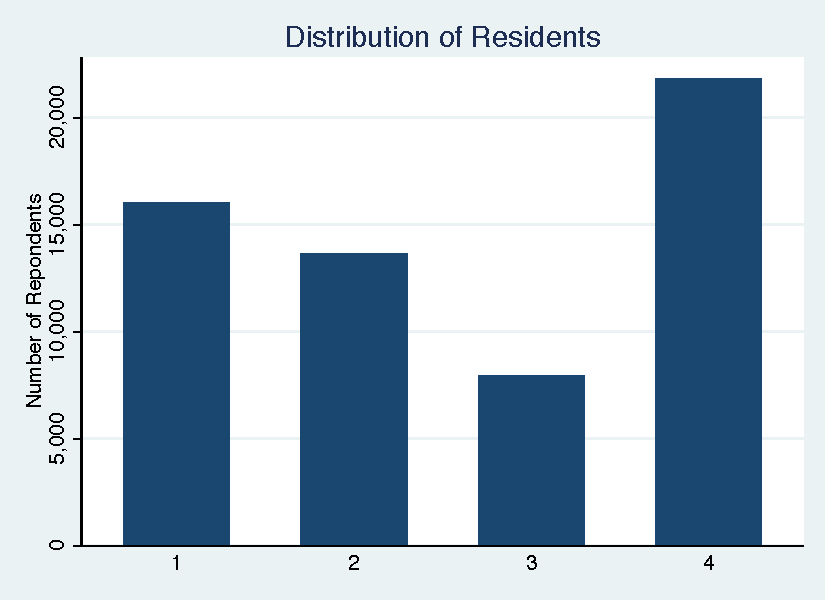
\includegraphics[width=\textwidth]{Residents}}
	\caption{\tb{Distribution of Responses By Place of Residence}}\label{figure1}
\end{figure}


\begin{figure}[ht!]    \centering
	{	 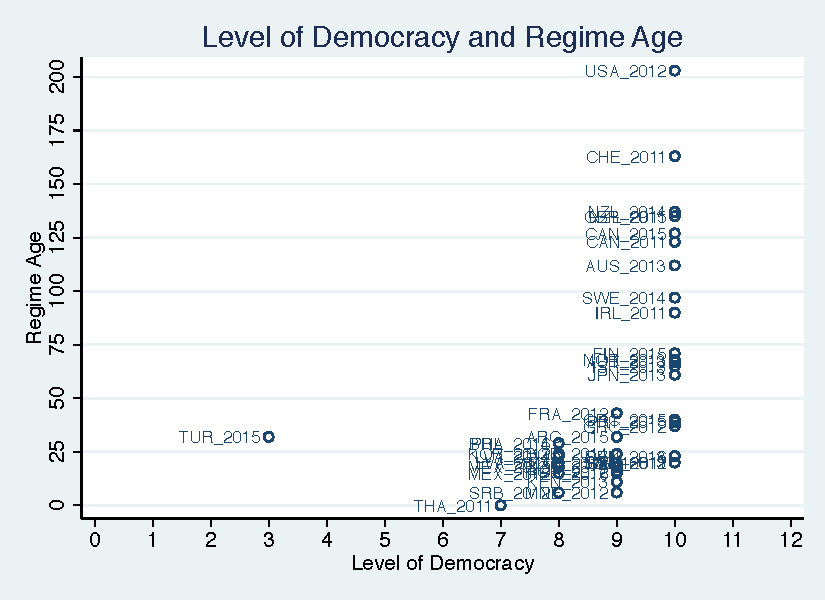
\includegraphics[width=\textwidth]{DemAge}}
	\caption{\tb{Level of Democracy and Regime Age}}\label{figure2}
\end{figure}

Now that we've analyzed the distribution of respondents by polity and the elections that the country is having in the studied election cycle, it is also beneficial to note some of the macro trends that are present which can help categorize the countires and take their variations into account in the analysis. Figure \ref{figure2} shows a graphical display of the countries represented in Module IV of the CSES sorted by their level of democracy and regime age. As the graph suggests, most of the countries represented in this study are very free. Yet, when it comes to the time that the electoral democracy has been around, most reside under the 50 year mark but it largely centers around and below 25 years. For a better breakdown of the exact values of each country's regime age and level of democracy, Table \ref{table101} in Appendix \ref{AppendixC} shows this data broken down more specifically, adding the consideration of the regime's electoral formula. From what this figure can show us, it is important to note some extreme values on both variables. Turkey's 2015 election stands out on Figure \ref{figure2} because it is the least democratic of the group. Additionally, it is also interesting to note the longest standing democracies such as the United States, Switzerland, Australia, Canada and New Zealand. These countries are those where there are most prior research given the country's openness to gathering of data from its citizens and the people's abilities to express their desires freely. The countries that center around eight and nine on the democracy scale that have democracies that are younger than 50 years will be the most interesting to consider given limitations in the existing literature that is available for these places.

\subsection{Proceeding with Caution}

As seen in previous works in American and Canadian politics, political parties are useful tools to predict votes since they are relatively useful heuristics that can assist in the formation of voting blocs. However, as \cite{holloway_burning_2007} notes, place of residence is not uniform throughout the world and it's people should not be treated as such. Rural voters are not voting blocs even if they can be seen to have similar voting patterns that span across a period of time. Yet, while some conceptualize a group under one light, it is not entirely the most accurate description of the way this group operates. Therefore, in answering the question of how place of residence influences political attitude formation, I aim to understand the general trends that happen in the world as a whole, but also within the boundaries of each country. I wish to tap into underlying mechanisms that can provide insight to why these trends exist and its repercussions in the hearts and minds of fellow citizens. I do not aim to make voting predictions about a country's next election; rather, I seek to understand if living in a place, on average, influences vote choice based on availability of social resources and activation of personal interests. With each of the conclusions I draw, the literature suggests that there are variations and other noise factors that should be considered before seeking to make generalizations about the rural or urban place of residence as a whole.

\section{Hypotheses}

From the review of literature, we see that there seems to be an ideological divide between people living in rural and urban areas of their respective countries. From case studies, most notably in the United States and Canada, there is a pattern such that the individuals living in rural areas tend to err towards conservatism and residents of urban centers tend to veer towards liberalism. However, given that these are relatively established democracies, I wonder how differences in levels of democratic development, regime age and other idiosyncratic factors that shape a regime influence the divide of political ideologies between urban and rural residents. Therefore, the present research will test three hypotheses relating to the relationship between the place of residence of an individual and their political ideology. For each of the following hypotheses, I address them as they speak to the average trends but also specific trends for each country analyzed.

\begin{quote}
	\e {Hypothesis 1 -- Place Matters:} An individual's place of residence influences their political ideology such that the more distant the characteristics of one's vicinity gets from an urban city, the more conservative one will become.
\end{quote}

The \e{Place Matters} hypothesis suggests that there is a direct relationship between place of residence and political ideology no matter where an individual lives in this world. Therefore, this hypothesis assumes that, broadly speaking, individuals who live in a rural area will be more conservative than those who live in a small town or urban center. In this case, political ideology, as we will also see later, is operationalized by the respondent's self-placement on the ideology spectrum. Therefore, this is based on their own views on how liberal or conservative they are. While this is helpful to understand how place of residence influences political ideology, it would be even more helpful to introduce a second hypothesis that looks at objective support for policies which can show where a person lies on the political spectrum.

\begin{quote}
	\e{Hypothesis 2 -- Issue Stances:} An individual's place of residence influences the way they conceptualize pressing issures and their stances towards these issues.
\end{quote}

In the \e{Issue Stances} hypothesis, I predict that people will understand the meaning of issues differently based on where they live and hold different opinions about them as a result of their place of residence. In other words, if the \e{place Matters} hypothesis holds true, people who live in rural areas will see issues differently than those who live in urban areas and apply their political ideologies when deciding on the issues. 

Both the \e{Place Matters} and \e{Issue Stances} hypotheses assumes that countries are the same across the board and that one's conceptualization of place of residence is uniform. Therefore, in the last hypothesis, I will integrate some polity defining factors into the model to understand how certain aspects of each regime such as their level of democracy, regime age and electoral formula influence the relationships that are observed in the preceding hypotheses. 

\begin{quote}
	\e{Hypothesis 3A -- Level of Democracy:} A regime's level of democracy will influence the political ideologies of citizens based on their place of residence such that the influence of place on political ideology will increase as a regime becomes more democratic. 
	
	\e{Hypothesis 3B -- Regime Age:} A regime's age will influence the political ideologies of citizens based on their place of residence such that the relationship between place of residence and political ideology will be more pronounced when the regime is older
	
	\e{Hypothesis 3C -- Electoral Formula:} A regime's method of elections will influence the political ideologies of citizens based on their place of residence such that pluralistic, first past the post systems will increase the influence of place of residence on political ideologies.
	
	\e{Hypothesis 3D -- Polity Differences} The regime's level of democracy, age and electoral formula will cooperate to determine the extent to which place of residence can influence political ideology in a given polity.
\end{quote}

Each of the components embedded in Hypothesis 3 analyzes key differences in how each polity functions and the stability of democracy such that a more stable democracy can mean more room for an individual to consider their true self-interests rather than being forced to believe something as a means of survival. In each of the sections of Hypothesis 3, we analyze how the successful consolidation of democracy, or lack thereof, influences how other social factors, such as place of residence, can influence a person's political views. I include the age of the regime to identify if a longer lasting polity can solidify the patterns of influence that place of residence has on an individual's political outlook and stance on issues. 

Finally, I include the electoral formula as a means of understanding how the system of representation influences the relationship between the core variables used in this paper. A regime's electoral formula is the way in which citizens select their representatives and the mechanisms in which votes are tallied. It is unclear whether the electoral formula influences political discourse and attitude formation. however, past research suggests that this factor does not matter in the ways that place of residence will influence a person's political preference \cite{barkan_space_2006}. For the \e{Electoral Formula} hypothesis, I hypothesize that if individuals had to fight for representation in a winner take all system, personal factors such as place of residence will be more salient than if all interests were more fairly represented in a proportional system. Each of these components are then tied together to understand how idiosyncrasies of a polity lead to the difference between place of residence and political ideology as explored in the \e{Place Matters} and the \e{Issue Stances} hypotheses.

Through the research, we will be able to see whether there is a relationship across the globe surrounding place of residence and political ideology. In the following sections, I explain the models that will be used to understand the relationships between the variables. We will revisit the hypotheses in the discussion to see if the data supports them along with possible limitations that may be present.

\section{Research Design}

\subsection{Data}

To understand the divide between rural and urban residents in different countries of the world, I will consider cases analyzed in the Comparative Study of Electoral Systems (CSES) Module IV dataset for the analysis of these trends. In this specific module, the CSES considers elections that occurred between 2011 and 2016 in various democracies around the world. In the following sections, I will describe the variables used in this project in more detail. Each of the variable names and descriptions are also located in Appendix \ref{AppendixA}, which contains the variable code referenced in the CSES dataset.

\subsection{Key Independent Variables}

In this data analysis, the key independent variables that are considered include the respondent's country and place of residence. For this analysis, place of residence is considered to be based on the categories that are established by the survey such that individuals either live in a rural village, small town, suburbs of a large city or within the large city itself. In the regression model, this variable is characterized as a category even though there are places that may be in between two of the categories that characterize place of residence. 

Each individual's country of residence is also classified based on the year of the election, level of democracy during the election year,  age of the current governing regime in the country at the time of the election, and the type of electoral formula employed by the governing body to determine winners of seats in government. The level of democracy is characterized by how free the polity is at the time of the election. This measure was gathered from the generators of the Polity IV project and reflects freedom from a -10 to 10 scale with -10 being the most autocratic and 10 being the most democratic. The age of the current governing regime suggests how long the current system has been in power. The larger value suggests that the current system in government has been established for a longer period of time and is therefore more stable. Finally, the type of electoral formula describes how government official win office based on their total vote share. Contestants may win via majoritarian, proportional or mixed system. 

\subsection{Key Dependent Variables and Measures}

To understand where individuals see their own political values, the dependent variable reflects their self-identified ideology, a variable coded by the CSES that ranges from 0 to 10 with 0 being the most left leaning and 10 as the most right leaning ideological stance.. Since this can be rather subjective, i also created a liberalism scale that reflects individual values on government spending with a more liberal vision being those who value spending for social benefits and a more conservative view for those who do not with for such spending or for those who wish to spend more to boost defence as a means to secure their country's identity and values. (See Appendix \ref{AppendixB} for a more detailed description of this scale creation) This 9-point scale was generated from questions relating to public expenditure used in the survey. Topics for these questions include health, education, unemployment benefits, defense, old age pensions, business and industry investments, police and law enforcement and welfare benefits. Additionally, I add a value of economic equality to the measure as a means of understanding how each person values equality as part of their ideological outlook. This scale ranges from 0 to 9, with 0 being the most conservative and 9 being the most liberal. In the broadest context, respondents who score at the extreme ends of the scale are seen to be most conservative or liberal in terms of their outlook on spending, which can speak to their views on social values given their willingness to allocate government money to these groups.

\subsection{Models for Analysis}

In this study, I will utilize five different regression analyses for each of the two dependent measures to uncover patterns in the data and help answer the guiding questions posed in the introduction. I will utilize the variables discussed in the previous sections to find connections between place of residence and political ideologies.

The first regression will consider the core of the \e{Place Matters} hypothesis. I will regress the place of residence variable on the respondent's self-placement on the political ideology scale. The second, third and fourth regressions will factor in the effects of a country's level of democracy, regime age, and electoral formula at the time of the election into the picture to observe their influences on the relationship in the \e{Place Matters} hypothesis. A fifth regression will be employed to understand how the inclusion of all the variables influences the first hypothesis. These subsequent hypotheses are aimed at testing the components of Hypothesis 3.

Hypothesis 2, or the \e{Issue Stances} hypothesis, is constructed as an objective measure and check to the subjective ratings. The Liberalism scale will be a dependent measure on another series of regressions that mirror the first set. The major difference with this set of regressions from the preceding set is the differences in dependent measure such that the former is based on how individuals think they are placed on the political ideology spectrum based on self-judgment, the latter is the measure of ideology based on the individual's actual policy stances.

In the following section, I discuss the results for the regressions and comment on the observations that these regressions can suggest for the relationship between place of residence and political ideology across a sample of countries across the world.

% Cross tabulate liberalism and self ideology to see how the two line up
\section{Results}


\subsection{Self-Placement Ideology as a Dependent Measure}

\subsubsection{\e{Place Matters} on the Worldwide Scale}

For the first model, a regression was conducted to see if there is a general trend between place and self-placement on a 10-point ideology scale. Furthermore, the regression was conducted separately for each election that was represented in this dataset. Table \ref{table3} shows the results for this regression on the global scale. This general trend suggests that, without considerations of any polity-specific factors, there is a difference between the global rural residents, small town and suburban residents in terms of their political ideologies. The trends described in this table suggests that, on a general level, there lies a difference between where people live and their political attitudes. However, several caveats are present in this analysis. From here, we are assuming that individuals conceptualize the places of residence in a similar fashion across geographic boundaries. Additionally, this analysis does not take into account country-specific measures such as the presence of the different possibilities of residence for the people. As I noted in Tab;e \ref{table2}, not all the countries have respondents from each place of residence as categorized in the CSES. Therefore, it would help to break down the analysis by country.

\begin{table}[H]
	\centering
	%\def\arraystretch{1.5}
	\caption{\tb{Self-Placement Ideology - Worldwide}}
	\begin{tabulary}{\linewidth}{l c}
		\\
		\hline
		\tb{Place of Residence}&\tb{Worldwide} \\
		\hline
		Small Town&-.1338***  \\    
		  & (.0336)   \\
		Suburban & -.2591***\\ 
		 & (.0358) \\
		Urban   & -.0482   \\
		  & (.0300)    \\
		Constant   & 5.597***  \\
		&(.0234) \\
		N  & 47,821  \\
		$R^2$	& 0.0011 \\
		\hline                                       
    \end{tabulary}
\\
\e{Notes:} *p$<$.1, **p$<$.05. ***p$<$.01 \\
\e{Reference:} A rural place of residence serves as the baseline for comparison
\label{table3}
\end{table}

\subsubsection{\e{Place Matters} By Geographic Region}

When the analysis is broken down by the countries themselves, we see a clearer patterns between place of residence and political attitudes of the respondents to the CSES survey. Each country is displayed and analyzed with their regional neighbors. Additionally, these trends are discussed in context of some key macro variables present for each polity that is displayed in Figure \ref{figure2} and Appendix \ref{AppendixC}.

Table \ref{table4} discusses the patterns seen by place of residence for countries in Central America and Latin America. From the results of the regression, we see that urban residents in Argentina are, on average, more liberal than their rural counterparts. This is slightly the case for Mexico at the time of their 2015 elections, but we do not see these trends elsewhere. When considering the levels of democracy, electoral formula and regime age for these countries, the notable difference between the regimes is the age of the system. Residents of Argentina have been living in a democracy for a longer period of time than the other countries represented in this region. 

\begin{table}[H]
\centering
%\def\arraystretch{1.5}
\caption{\tb{Self-Placement Ideology - Central/Latin America}}
	\begin{tabulary}{\linewidth}{l c c c c}
	\\
	\hline
	\tb{Place of Residence}&\tb{Argentina}&\tb{Mexico (2012)}&\tb{Mexico (2015)} &\tb{Peru}\\
	\hline
	Small Town  & -    & .6408***   &-.4734    & -   \\      
	  & -  & (.2394) & (.3113)    & -    \\
	Suburban    & -    & -   & -   & -    \\ 
	& -     & -    & -   & -    \\
	Urban   & -.9521*** & -.1417   & -.4084*   & .0883  \\
	   & (.2150)   &(.1678)   & (.2210)  & (.1743)      \\
	Constant   & 6.495*** & 6.6516*** & 6.1690*** & 6.646***   \\
	&(.2046)&(.1493)&(.1998)&(.1564) \\
	N  & 1,241 &1,812   & 910 & 1,438   \\
	$R^2$ & 0.0156   &0.0082   &0.0041 &0.0002     \\
	\hline                                       
	\end{tabulary} 
\\
\e{Notes:} *p$<$.1, **p$<$.05. ***p$<$.01 \\
\e{Reference:} A rural place of residence serves as the baseline for comparison
\label{table4}
\end{table}

In Western Europe, as Table \ref{table5} shows, there is a clearer divide between place of residence and political ideologies, such that, for all of the counties displayed in the table, urban residents are significantly more likely to be more left-leaning than their rural counterparts. Additionally, suburban residents in Switzerland and Portugal are also more likely to be more left-leaning than their rural counterparts. Small town residents can be slightly more left-leaning than rural residents in Portugal, Great Britain and Germany. The countries in this region are some of the free-est and oldest democracies in the world. Therefore, individuals here have had a longer time to socialize and develop their opinions based on factors relating to self-interest. 

\begin{landscape}
\begin{table}
	\centering
	\def\arraystretch{1.5}
	\caption{\tb{Self-Placement Ideology - Western Europe}}
	\begin{tabulary}{\linewidth}{l c c c c c c}
		\\
		\hline
		\tb{Place of Residence}&\tb{Switzerland}&\tb{Germany}&\tb{France} &\tb{Great Britain}&\tb{Ireland}&\tb{Portugal}\\
		\hline
		Small Town   & - .4973  & -.3295*** &-.1148 &  -.3773***  & -   &-.3717* \\      
		& (.4333)  & (.1087)  & (.1321)    & (.1392)  &- & (.2157) \\
		Suburban  & -.2663***   & .0912 & -.0246  & -      &-    & -1.1139*** \\ 
	    & (.0852)  & (.1693)  & (.1886)   & -      & - & (.2421)  \\
		Urban  & -.8650***  & -.6361*** & -..7254***  & -.8310***      &-.2494**& -.8348***   \\
	    & (.0976)  &(.1311)  & (.1706)    & (.1538)   & (.0986)  & (.2121)  \\
		Constant & 5.462***  & 4.630***  & 4.8086***  & 5.3992***  & 6.1491***  &5.4661***   \\
		&(.0681)&(0.0845)&(.0943)&(.1197)&(.0772)&(.1483) \\
		N  & 4,728    &1,697  & 1,916  & 1,386     &  1,594  &1,224  \\
		$R^2$  & 0.0191    &0.0176 &0.0102    &0.0217  &  0.0040 &0.0218  \\
		\hline                                       
	\end{tabulary} 
	\\
	\e{Notes:} *p$<$.1, **p$<$.05. ***p$<$.01 \\
	\e{Reference:} A rural place of residence serves as the baseline for comparison
	\label{table5}
\end{table}
\end{landscape}

Countries in Northern Europe are also relatively free in terms of their level of democracy and time that such democracy is established. Like their Western European counterparts, Scandinavian countries hold similar governing systems but do not experience similar trends in terms of place of residence and political attitudes. As Table \ref{table6} suggests, Finland is the only country with a sharp urban-rural divide. Iceland's place divide comes with the suburban-rural split between the residents. While there are subtle levels of significance elsewhere, it is clear that there is a regional difference when it comes to how democracy influences individual's political attitudes based on place. In the light of countries of Western Europe, Northern European countries do not see the same patterns fo residence divides even with similar freedoms and levels of democracy. This suggests that there are other differences in these regions that are worth considering.

\begin{table}[H]
	\centering
	%\def\arraystretch{1.5}
	\caption{\tb{Self-Placement Ideology - Scandinavia}}
	\begin{tabulary}{\linewidth}{l c c c c}
		\\
		\hline
		\tb{Place of Residence}&\tb{Finland}&\tb{Iceland}&\tb{Norway}&\tb{Sweden} \\
		\hline
		Small Town&.1418&.5194**&.0568&-.1030 \\
		&(.1646)&(.2279)&(.1534)&(.2644) \\
		Suburban&-.0612&.7355***&-.0277&.0794 \\
		&(.1452)&(.2290)&(.1847)&(.2690) \\
		Urban&-.7128***&.3840*& .0888&-.1723\\
		&(.2202)&(.2220)&(.1429)&(.2368) \\
		Constant&5.6503***&4.990***&5.5985***&5.2230*** \\
		&(.1169)&(.2006)&(.1080)&(.1973) \\
		N&1,387&1,266&1,618&792\\
		$R^2$&0.0111&0.0096&0.0004&0.0018 \\
		\hline
	\end{tabulary}
\\
\e{Notes:} *p$<$.1, **p$<$.05. ***p$<$.01 \\
\e{Reference:} A rural place of residence serves as the baseline for comparison
\label{table6}
\end{table}

Turning to Central Europe, Table \ref{table7} suggests that there is a significant difference between place of residence and political attitudes in Slovenia and Slovakia. When we consider factors such as level of democracy and regime age as we did previously, freedom by democracy and stability of the regime are not necessarily trends that help shape the influence of place of residence and political ideologies here. As we previously established, it seems that the oldest regimes in each region lead to more pronounced differences between rural and urban residents, but this trend is not necessarily the case here. Austria is the oldest regime in the region, but urban residents are only slightly more left-leaning than their rural counterparts. 

\begin{table}[H]
	\centering
	%\def\arraystretch{1.5}
	\caption{\tb{Self-Placement Ideology - Central Europe}}
	\begin{tabulary}{\linewidth}{l c c c c c}
		\\
		\hline
		\tb{Place of Residence} &\tb{Austria}&\tb{Czech Republic}& \tb{Poland} &\tb{Slovakia}&\tb{Slovenia} \\
		\hline
		Small Town&-.2108& -.0223 & .0829 & .4318*** & .0229 \\
		&(.1540) & (.1687) & (.1421) & (.2000) & (.3262)\\
		Suburban&-.1433& -.6091*& -.1414 & 1.059& .1549** \\
		&(.1570)&(.3281) & (.2210) & (.6711) & (.2491)\\
		Urban&-.3005**&.2860 & -.2002 & .8061*** & -1.3416***\\
		&(.1335) &(.1773) & (.2042) & (.2437) & (.3169)\\
		Constant& 5.3726***& 4.9135***& 6.015*** & 4.7527***  & 4.6780 ***\\
		&(.1219) & (.1300) & (.1050) & (.1370) & (.2060)\\
		N&3,363& 1,412& 1,634 & 879& 666 \\
		$R^2$&0.0018&0.0065 & 0.0016 & 0.0148 & 0.0629\\
		\hline
		\end{tabulary}
	\\
	\e{Notes:} *p$<$.1, **p$<$.05. ***p$<$.01 \\
	\e{Reference:} A rural place of residence serves as the baseline for comparison
	\label{table7}
	\end{table}

In Southwestern Europe, the countries, especially those represented by two separate elections, suggest that trends in the influence of place of residence vary by election. This pattern is perhaps the clearest to discern in this region given that there are more countries here with multiple elections represented in the present module of the dataset. In Greece and Romania, we see that the urban-rural divide was present in the former but not the latter of the elections. This can be attributed to other factors such as candidates who are running in that particular race or the policies that are the most salient in the region at the time. Table \ref{table8} shows these trends and also suggests that Bulgaria and Montenegro see trends of rural-urban division.

\begin{landscape}
\begin{table}
	\centering
	\def\arraystretch{1.5}
	\caption{\tb{Self-Placement Ideology - Southwestern Europe}}
	\begin{tabulary}{\linewidth}{l c c c c c c c}
		\\
		\hline
		\tb{Residence}& \tb{Bulgaria}& \tb{Greece ('12)}& \tb{Greece ('15)} & \tb{Montenegro} & \tb{Serbia} & \tb{Romania ('12)} & \tb {Romania ('14)}\\
		\hline
		Small Town&.5324 &-.7220*** &-.1458 & -1.3499*** & .2226 & .1211 & .2699\\
		&(.3313)& (.2656) & (.3484) & (.3282) & (.2098)& (.2304) & (.3097)\\
		Suburban& .7821*** & -1.058*** &-.0685 & -.9444** &.1046 &-.1422 &.1463\\
		& (.2914) &(.2557) & (.3667) & (.4876) &(.2900) & (.5737) & (.4000)\\
		Urban& .8838**& -1.1088*** & -.1737 & -1.4676*** & -.1549 & .7782*** & -.3691\\
		& (.3590)& (.1797) & (.3236) & (.4987) & (.2437) & (.2105) & (.3712)\\
		Constant& 4.739*** &5.5410*** & 4.5961*** &6.7329*** & 5.4643*** & 4.7229*** & 6.4406***\\
		& (.2267) & (.1271)  & (.3089) & (.2409) & (.1239) & (.1438) & (.1890)\\
		N& 750 & 928 & 905 & 450 & 1,094 & 1,192 &714\\
		$R^2$&0.0118 &0.0441& 0.0005 &0.0419 & 0.0020 & 0.130 &0.0037 \\
		\hline
	\end{tabulary}
\\
\e{Notes:} *p$<$.1, **p$<$.05. ***p$<$.01 \\
\e{Reference:} A rural place of residence serves as the baseline for comparison
\label{table8}
\end{table}
\end{landscape}

Yet, not all countries experience patterns of changing urban-rural division between elections. In Eastern Europe, as represented by Latvia in Table \ref{table9}, the country did not see a shift in attitudes for respondents based on a change in election. 

\begin{table}[H]
\centering
	%\def\arraystretch{1.5}
	\caption{\tb{Self-Placement Ideology - Eastern Europe}}
	\begin{tabulary}{\linewidth}{l c c}
		\\
		\hline
		\tb{Place of Residence} & \tb{Latvia (2011)} &\tb{Latvia (2014)} \\
		\hline
		Small Town &.1635 &.0560 \\
		&(.2433) & (.2224) \\
		Suburban&- & -.1285 \\
		& - & (.2893) \\
		Urban&-.2292&.0221 \\
		& (.1850) & (.1996) \\
		Constant & 6.2775*** &6.3285*** \\
		& (.1360) & (.1396) \\
		N&787 & 815\\
		$R^2$& 0.0041 &0.0005 \\
		\hline
	\end{tabulary}
\\
\e{Notes:} *p$<$.1, **p$<$.05. ***p$<$.01 \\
\e{Reference:} A rural place of residence serves as the baseline for comparison
\label{table9}
\end{table}

For the data that is available to the Middle East, Africa and Asia, there are simply not enough cases here to make general arguments about the region as a whole. Nonetheless, they are still useful in helping us to understand which countries have a sharper urban-rural divide.

To start, Table \ref{table10} highlights Israel as a country in the Middle East with sharp urban and suburban divides to the rural areas of the country in terms of its political ideology. This is not an effect that is seen in Turkey. A reason for this trend is the freedoms that the people in these countries experience. While it is hard to tell if this pattern is true for all countries in the region, it is worth noting that the differences in the level of democracy here may have a great influence in individual political attitudes. Like the actors in Western Europe and much of the western, democratized world, Israel stands as one of the freest nations in the region. Their democracy has been established for 60 years at the time of this election. Meanwhile, Turkey is the least free of all of the countries that are surveyed in this Module. This limit in freedom of speech at the ballot box may also lay to limit freedom of association and expression for the people in the country, limiting the influence of one's vicinity and social group influence on one's political attitudes.

\begin{table}[H]
	\centering
	%\def\arraystretch{1.5}
	\caption{\tb{Self-Placement Ideology - Middle East}}
	\begin{tabulary}{\linewidth}{l c c}
		\\
		\hline
		\tb{Place of Residence}&\tb{Israel} & \tb{Turkey} \\
		\hline
		Small Town&1.2822*** & .0228 \\
		&(.2427)  & (.3120)\\
		Suburban&1.5019*** &.5457 \\
		& (.2767)  & (.3326 )\\
		Urban &- & .2337\\
		&- & (.2764)\\
		Constant& 4.9193*** &5.7434*** \\
		& (,.2067)  & (.2268)\\
		N&912 & 965\\
		$R^2$&0.0371 & 0.0037 \\
		\hline 
	\end{tabulary}
\\
\e{Notes:} *p$<$.1, **p$<$.05. ***p$<$.01 \\
\e{Reference:} A rural place of residence serves as the baseline for comparison
\label{table10}
\end{table}

In the wake of the decolonization movement, countries in Africa are rather young in terms of the length of time that their democracy has been in place. In both of the cases displayed in Table \ref{table11}, it does not seem that the age of the democracy is the reason that place is likely to influence political ideology like other regions in the world. Kenya, a younger regime than South Africa, has a greater difference between urban and rural residents such that urban residents are more likely to be left-leaning at a larger factor (1.269 points on average to the left) than in other places in the world. 

\begin{table}[H]
	\centering
	%\def\arraystretch{1.5}
	\caption{\tb{Self-Placement Ideology - Africa}}
	\begin{tabulary}{\linewidth}{l c c}
		\\
		\hline
		\tb{Place of Residence} & \tb{Kenya}& \tb{South Africa} \\
		\hline
		Small Town&- &-\\
		&- & -\\
		Suburban&- & -\\
		& - &- \\
		Urban&-1.2690*** &-.06719 \\
		&(.3701)  &(.1664)\\
		Constant&6.7690*** &6.4965*** \\
		& (.1932) & (.1392) \\
		N&506 & 967\\
		$R^2$&0.0228 &0.0002 \\
		\hline
	\end{tabulary}
\\
\e{Notes:} *p$<$.1, **p$<$.05. ***p$<$.01 \\
\e{Reference:} A rural place of residence serves as the baseline for comparison
\label{table11}
\end{table}

In this sample of countries from Asia, the data in Table \ref{table12}, suggests that neither Japan nor South Korea exhibit a significant trends towards having place influence a person's placement on the left-right scale. This is also visible in countries in the Pacific Island, and Australia. But in the cases of the countries displayed in table \ref{table13}, the more democratic a place is does not necessarily suggest that there is a greater division between urban and rural residents in terms of their political ideologies. The Philippines, for instance, is less free than Australia and New Zealand, but demonstrate a greater place divide in terms of political ideology.

\begin{table}[H]
	\centering 
	%\def\arraystretch{1.5}
	\caption{\tb{Self-Placement Ideology - Asia}}
	\begin{tabulary}{\linewidth}{l c c}
	\\
	\hline
	\tb{Place of Residence} & \tb{Japan} & \tb{South Korea}\\
	\hline
	Small Town &.1898 & -.0347 \\
	&(.1463) & (.2738 )\\
	Suburban&.1717 & -.1176 \\
	& (.1574) & (.4343 )\\
	Urban & .2429* &.3140 \\
	& (.1365) & (.2518)\\
	Constant& 5.4179*** & 5.264*** \\
	& (.1210) & (.2158)\\
	N&1,563 & 717\\
	$R^2$& 0.0020 & 0.0052\\
	\hline
	\end{tabulary}
\\
\e{Notes:} *p$<$.1, **p$<$.05. ***p$<$.01 \\
\e{Reference:} A rural place of residence serves as the baseline for comparison
\label{table12}
\end{table}

\begin{landscape}
\begin{table}
	\centering
	\def\arraystretch{1.5}
	\caption{\tb{Self-Placement Ideology - Pacific Islands}}
	\begin{tabulary}{\linewidth}{l c c c c}
		\\
		\hline
		\tb{Place of Residence}&\tb{Australia}&\tb{New Zealand (2011)}&\tb{New Zealand (2014)} &\tb{Philippines}\\
		\hline
		Small Town  & - .2108  & -.2283  &-.1436 &  .6419***  \\      
		& (.1540)   & (.2213) & (.2864)  & (.2060)    \\
		Suburban  & -.1433   & -   & -    & - .1095   \\ 
		& (.1570)   & -  & -    & (.3871)       \\
		Urban  & -.3005** & -.2653  & -.2151 & .3048** \\
		& (.1335) &(.2114)   & (.2406) & (.1526)      \\
		Constant   & 5.372***   & 5.754*** & 5.9674***  & 7.009***   \\
		&(.1219)&(.1826)&(.2207)&(.1030) \\
		N 	 & 3,363   &1,039    & 957   & 1,179  \\
		$R^2$  & 0.0018   &0.0016  &0.0035  &0.0097     \\
		\hline                                       
	\end{tabulary} 
	\\
	\e{Notes:} *p$<$.1, **p$<$.05. ***p$<$.01 \\
	\e{Reference:} A rural place of residence serves as the baseline for comparison
	\label{table13}
\end{table}
\end{landscape}

\subsubsection{Summary: Place Matters?}

In our analysis for the influence of place of residence on the political attitudes of individuals in certain countries of the world, we generate rather mixed conclusions based on the data. When we consider the differences between neighboring countries in terms of differences in regime age and level of democracy, these factors, nonetheless produce mixed results as an answer to the question about whether place matters in influencing political ideology. From the overall trends, we have evidence to suggest that place of residence does matter, but it depends on contextual factors that extend beyond the information that a country's regime stability, as determined by age, and the freedoms people enjoy, as determined by level of democracy, can tell us about the underpinnings of these observations.

\subsection{Objective Issue Stances as a Dependent Measure}

In the previous section, I looked at specific countries to try to discern the extent to which place matters in a person's self placement on the political ideology spectrum. From the results of that model, we can see that place matters, but the country to which the place is embedded in also matters to determine and influence the relationship between the variables. In this section, I aim to explore a more objective variable on liberalism to see the extent to which place really matters in influencing individual political attitudes towards economic and social inequality. As previous research suggests (notably, \cite{walsh_putting_2012}), residents of rural environments tend to be more conservative when it comes to social spending, even if the results will work in their favor. 

The analysis employed in this section will look at general trends to see if there is indeed an influence between place and positions on spending. A variable was created for this analysis which aggregates the views that people have for spending government money on various social services in the country (see Appendix \ref{AppendixB} for more information on variable coding). 

\begin{table}[h!]
	\centering
	%\def\arraystretch{1.5}
	\caption{\tb{Issue Stances - General Trends}}
	\begin{tabulary}{\linewidth}{l c}
		\\
		\hline
		\tb{Place of Residence} & \tb{Worldwide} \\
		\hline 
		Small Town&-.1005*** \\
		&(.0136)\\
		Suburban&-.1737***\\
		&(.0162) \\
		Urban&-.1306*** \\
		&(.0123)\\
		Constant&5.7164*** \\
		&(.0093) \\
		N&42,500 \\
		$R^2$&0.0037 \\
		\hline
	\end{tabulary}
	\\
\e{Notes:} *p$<$.1, **p$<$.05. ***p$<$.01 \\
\e{Reference:} A rural place of residence serves as the baseline for comparison
\label{table14}
\end{table}

From the results that reflects general trends in the world based on the new liberalism variable, we see that there are some differences between place of residence and issue stances. Looking at Table \ref{table14} alongside the earlier Table \ref{table3}, we see that there urban-rural divide is more pronounced than it was before. (Both Tables are reproduced in Appendix \ref{AppendixD} for simplicity in comparison)

However, the results here provide an interesting deviation from the patterns that are observed using self-placement on the ideology spectrum as a dependent variable. Here, a higher score indicates that individuals will be \e{more} liberal when it comes to government spending on social policy. As noted earlier, residets of urban centers tend to see themselves as more left-leaning, but they are relatively less interested in seeing government spend more money on health care, defense, and other social welfare measures that would ensure equity among the people in the country.

\subsection{Considerations of Regime Age,, Level of Democracy, and Electoral Formula}

In the analysis of results for self-placement ideology, we considered if a country's macro variables has any influence on the relationship between place of residence and political ideology.

To test the core of Hypothesis 3, we will turn next to how these macro variables influence the context where each respondent casts their ballot. I will analyze the big picture before diving into the specifics regarding each factor. Therefore, we will look at the \e{Polity Difference} hypothesis before diving into \e{Level of Democracy}, \e{Regime Age}, and \e{Electoral Formula} hypotheses.

Table \ref{table15} shows the influence of each of the macro variables, when taken together, on the relationship between place of residence and individual placement on political ideology and on the objective measures seen in the liberalism measure.

\begin{table}[h!]
	\centering
	%\def\arraystretch{1.5}
	\caption{\tb{All Macro Variables - General Trends}}
	\begin{tabulary}{\linewidth}{l c c}
	\\
	\hline
	\tb{Variable}&\tb{Self-Placement}&\tb{Liberalism} \\
	\hline
	\e{Place of Residence} & & \\
	Small Town &-.1000***&-.0018 \\
	&(.0339)&(.0130) \\
	Suburban& -.1517***& .0147 \\
	&(.0401)& (.0157) \\
	Urban&-.0517* & -.0420*** \\
	&(.0304) & (.0117) \\
	\e{Democracy}& -.1995*** & -.0421***\\
	&(.0110) & (.0040)\\
	\e{Regime Age} & -.0014*** &  -.0075***\\
	&(.0002) & (.0001)\\
	\e{Electoral Formula}&.0778*** & -.0440***\\
	&(.0189) & (.0070) \\
	\hline
	Constant& 7.3627*** & 6.5149*** \\
	&(.1067) & (.0391)\\
	N&46,555 & 41,373 \\
	$R^2$&0.0135& 0.1273 \\
	\hline
	\end{tabulary}
	\\
\e{Notes:} *p$<$.1, **p$<$.05. ***p$<$.01 \\
\e{Reference:} A rural place of residence serves as the baseline for comparison
\label{table15}
\end{table}

The data in Table \ref{table15} suggests that there is a difference between urban and rurual residents when it comes to spending, but this pattern is not as emphasized in self-placement ideology. The results of this model confirms the work from previous literature to show that urban residents are more open to government spending to help a neighbor than residents in a rural area of a country. Yet, the interesting difference lies in the breakdown of self-placement on the ideology spectrum. While there is not as much significance between urban and rural residents, there are differences with each of the residence types that can be analyzed further.

For the purposes of simplicity in the forthcoming discussion, I will analyze the influence of both dependent variables, but primarily focusing on the self-placement of individuals on the ideology spectrum. From the previous discussion in this section, we can see that the major difference between the different places lie primarily in the self-placement score rather than the liberalism variable. While the objective score is interesting in its own ways, and it will be considered, the weight will be placed on how people see themselves and their place on the political spectrum. 

\subsubsection{By Level of Democracy}

A model that considers the interaction of a country's level of democracy and place of residence on an individual's political attitudes was conducted and the results suggests that the effect of place is more pronounced at lower levels of democracy. However, this is an effect that works in theory and not in practice. Countries with lower levels of democracy might have greater levels of divide between the quality of life in cities than suburbs than rural towns. This observation was displayed numerous times in previous analyses of polities where countries with lower levels of democracy were experiencing a greater difference between place and political attitudes, as exhibited in Asia. Yet, limitations in political expression might mask this reality, which suggests that further exploration in the data is necessary. 

Additionally, the regression suggests that countries with great levels of freedom, which includes the majority of the polities that are included in this study, do not have interactive effects with regard to level of democracy. In other words, this result suggests that having freedoms related to democracy are great, but there may be other factors that mitigates the differences between places of residence and political attitudes. When we looked at countries in each region, there are countries with similar level of democracy, but stark differences in the relationship of core variables.

\subsubsection{By Regime Age}

To understand the interaction between the age of a regime and place of residence on political ideology, I ran a regression to explore these effects. 

\subsubsection{By Electoral Formula}

For this section, we consider Electoral formula. Since there are only 3 categories that any country can select, it makes direct comparison more straightforward. Unlike the previous two discussions, this variable is not continuous, thereby making interactions not as suitable.

\begin{table}[h!]
	\centering
	\caption{\tb{Ideology In Each Electoral Formula}}
	\begin{tabulary}{\linewidth}{l c c c}
		\\
		\hline
		\tb{Place of Residence}&\tb{Majoritarian}&\tb{Proportional} &\tb{Mixed} \\
		\hline
		Small Town&-.6640*** &.0608 &-.1600** \\
		&(.0766)&(.0435) &(.0727) \\
		Suburban&-.6389*** &-.1894***&-.1260  \\
		&(.1042) &(.0451) &(.1180) \\
		Urban&-.5781*** &-.0327 &.2655*** \\
		&(.0710) &(.0388) &(.0644) \\
		Constant& 5.8256*** &5.5408***&5.5562*** \\
		&(.0543) &(.0297) &(.0531) \\
		Countries&5&21&6 \\
		N&8,350&28,869 &10,602 \\
		$R^2$&0.0114&0.0011 &0.0052 \\
		\hline 
	\end{tabulary} 
\\ 
\e{Notes:} *p$<$.1, **p$<$.05. ***p$<$.01 \\
\e{Reference:} A rural place of residence serves as the baseline for comparison
\label{table16}
\end{table}

Table \ref{table16} shows the relationship of place of residence in countries grouped by their electoral formula. By the differences in the results, we can see that the electoral formula matters in the relationship between place of residence and political attitudes.

Majoritarian elections are defined by first-past-the-post result tabulations where the candidate with the most votes is tapped as the winner of the race. With this campaign method, there is space of candidates to appeal to certain constituencies strategically to gain the most votes for themselves. In theory, a large representative body should serve different interests, but reality is hard to match expectations. Therefore, candidates and voters alike must push for their own interests to dominate, making a polarized electorate more likely on the lines of differing interest \cite{abramowitz-2010}. The results confirms this expectation. Individuals living in small towns, suburban and urban areas are significantly mor likely to lean left than their rural counterparts. While the differences among each other is not as big of a difference, it is significantly different from a rural place of residence. 

Proportional representation occurs when parties are able to allocate votes in ratio to the number of votes that they receive. Therefore, it becomes more likely that different interests are represented in practice and that minority parties will have a chance in policymaking. This may help explain the insignificant results for the differences in places of residence on political attitudes when the countries are aggregated. However, in our previous discussions, proportional countries also see significant differences between places of residence, with Israel and Greece in 2012. However, this aggregate pattern carries for most of the other proportional representation states in this study.

Finally, a mixed representation system has combinations of the aforementioned systems. When aggregated, there are differences between place of residence and political attitudes. Depending on the specifications of the government design in each country, there can be great variations between countries and levels of significance. While the urban-rural divide is significant in Germany, it is not so in Japan. 

To conclude, we see that the electoral formula matters in shaping political competition and electoral appeals from the perspective of the party. However, there are not clear distinctions for formulas such that it is a tell-all third factor in explaining the relationship between place and political attitudes. 

\section{General Discussion and Conclusion}

From the results of the data analyses, we can see that there are general relationships between place and political attitudes. However, when we dive deeper into the individuality of each country, we see that the idiosyncrasies that define each polity makes this a hard generalization to make. 

\subsection{Summary of Findings}

The goal of this paper is not to make generalizations about how people who live in suburbia around the world compare to those in the rural countryside when it comes to political attitudes, rather, it is to gain a general understanding of how the variables of place and political attitudes relate on a broad and specific level. From the data, I can draw the following conclusions. First, place matters. In the \e{Place Matters} hypothesis, the results confirm the findings such that urban residents, on average, differ from their rural counterparts when it comes to political ideology. The results confirm that urban residents, along with small town and suburban residents, tend to be more left leaning than their rural counterparts. However, the average difference between urban and rural, suburban and rural, and even small town and rural, are not necessarily increasing as one moves towards the city. Residents of the global suburbia, on average, see themselves to be more left leaning than their urban counterparts.

Second, the \e{Issue Stances} hypothesis is supported by the data because a person's place of residence does influence how one conceptualizes the issues and rate their support. However, as seen in Table \ref{table14}, urban residents are, on average, more conservative on their willingness to spend public dollars than their rural counterparts. This comes in contrast with the results in the \e{Place Matters} hypothesis. While urban residents may see themselves as more left leaning, they may have other motivations to limit their support for social and economic policy.

Finally, in Hypothesis 3, we examine the macro variables that are part of defining major democratic aspects of each country.

\subsection{Limitations and Future Directions}

For this project, that are many possible future directions that the research can go. In this section, I discuss how present limitations can become possible access points to future research and expansions of this paper.

As discussed throughout the analysis, each polity's idiosyncrasies cannot be fully accounted for in this one study. While this study is useful in understanding global trends, more research in the country's macro-variables are necessary to understanding why there is a significant relationship between place and political ideology in some counties and not others, even if they share grounds on level of democracy, regime age, and electoral formula.

The liberalism issue stance scale was created as a means of universalism, which was helpful in gaining some insight on how individuals conceptualize issue stances. However, it would be helpful to take the voting behavior of each participant into account and see how their self-rated political ideology compares to the candidate that they voted for in their legislative election. These specifications that are necessary to understand the differences between polities for the relationship of place and political attitudes provides insight as to why case studies have been the more popular method in analyzing these trends. 

While there is a relatively healthy mix of countries from different regime ages and electoral formulas, there is not an even distribution of countries based on their level of democracy. For future research, it would be helpful to include more transitioning regimes and autocratic regimes so long as public data is available. It is hard to gather data in their regimes due to government limitations, but trends in these sections would be interesting to observe.

Nonetheless, future research can be dedicated to looking at specifications that set each polity aside including historical, economical, political and other social factors. Residents of a certain place, as \cite{holloway_burning_2007} noted, are clearly not voting blocs. Unique factors of each country can help to explain the influence, or lack thereof, of place and political ideology better than how generalizations can tease out.       

\clearpage


\let\svaddcontentsline\addcontentsline
\renewcommand\addcontentsline[3]{%
	\ifthenelse{\equal{#1}{lof}}{}%
	{\ifthenelse{\equal{#1}{lot}}{}{\svaddcontentsline{#1}{#2}{#3}}}}


\appendixtitleon
\appendixtitletocon

\begin{appendices}
	
\section{Regimes Broken Down by Macro Variables}
\label{AppendixC}

\begin{table} [h!]
	\centering
	\caption{\tb{Regimes by Level of Democracy, Regime Age, and Electoral Formula}}
	\begin{tabulary}{\linewidth}{l c c c}
		\hline
		\tb{Country} & \tb{Level of Democracy} & \tb{Age of Regime} & \tb{Electoral Formula} \\
		\hline
		Argentina&9&32&Proportional \\
		Australia& 10&112&Majoritarian \\
		Austria&9&24&Proportional\\
		Bulgaria&8&24&Proportional\\
		Czech Republic&9&20&Proportional \\
		Finland&10&71& Proportional \\
		France&9&43&Majoritarian \\
		Germany&10&23&Mixed \\
		Great Britain&10&135&Majoritarian \\
		Greece (2015)&10&40&Proportional \\
		Ireland&10&90&Proportional \\
		Israel&10&60&Proportional \\
		Japan&10&61&Mixed\\
		Kenya&9&11&Majoritarian \\
		Latvia (2014)&8&23&Proportional\\
		Mexico (2015)& 8&18&Mixed\\
		Montenegro&9&6&Proportional\\
		Norway&10&68&Proportional\\
		New Zealand (2014)& 10& 137& Mixed\\
		Peru&9&15&Proportional\\
		Philippines&8&26&Majoritarian\\
		Poland&10&20&Proportional\\
		Portugal&10&39&Proportional\\
		Romania (2014) &9&18& Mixed \\
		Serbia& 8&6&Proportional\\
		Slovakia&10&23&Proportional\\
		Slovenia&10&20&Proportional\\
		South Africa&9&20& Proportional \\
		South Korea&8&24&Mixed\\
		Sweden&10&97&Proportional\\ 
		Switzerland&10&163&Proportional\\
		Turkey&3&32&Proportional\\
		United States&10&203&Majoritarian \\
		\hline
	\end{tabulary}
\\
\e{Source:} Polity IV Project and CSES Macro Report
\label{table101}
\end{table}

\clearpage 

\begin{landscape}
\section{Descriptions of Variables }
\label{AppendixA}

~~~\\\\

\begin{table}[h!]
	\centering
	\def\arraystretch{1.5}
	\caption{\tb{Variables Used in Analyses}}
	\begin{tabulary}{\linewidth}{l c c c}
		\\
		\hline
		\tb{Variable Name}& \tb{Variable Number} & \tb{Description}&\tb{Outside Source} \\
		\hline
		Election ID Variable &D1004&Polity and Election Year&-\\
		Place of Residence&D2031&Rural or Urban Residence&-\\
		Left-Right Self&D3014&Self-rate ideology &-\\
		Level of Democracy&D5051\_1&Democracy-Autocracy at Election&Polity IV Project\\
		Age of Current Regime&D5052&Age of Regime in Years& Polity IV Project\\
		Electoral Formula&D5058&Method of Election&CSES Macro Report\\
		\hline
	\end{tabulary}\\
	\e{Source:} Comparative Study of Electoral Systems Module IV Codebook available at \url{http://www.cses.org/datacenter/module4/data/cses4_codebook_part2_variables.txt}
	\label{table99}
\end{table}

\begin{table}[h!]
	\centering
	\def\arraystretch{1.5}
	\caption{\tb{Issue Stances/Liberalism Scale Variables}}
	\begin{tabulary}{\linewidth}{l c c c}
		\\
		\hline
		\tb{Variable Name}& \tb{Variable Number} & \tb{Description}\\
		\hline
		Health&D3001\_1&More or Less Public Expenditure on Health\\
		Education&D3001\_2&More or Less Public Expenditure on Education\\
		Unemployment Benefits&D3001\_3&More or Less Public Expenditure on Unemployment\\
		Defense&D3001\_4&More or Less Public Expenditure on Defense\\
		Old-Age Pensions&D3001\_5&More or Less Public Expenditure on Pensions\\
		Business and Industry&D3001\_6&More or Less Public Expenditure on Businesses\\
		Police&D3001\_7&More or Less Public Expenditure on Law-Enforcement\\
		Welfare Benefits&D3001\_8&More or Less Public Expenditure on Welfare\\
		Income Inequality&D3004&Should Government do more for Income Inequality?\\
		\hline
	\end{tabulary}\\
	\e{Source:} Comparative Study of Electoral Systems Module IV Codebook available at \url{http://www.cses.org/datacenter/module4/data/cses4_codebook_part2_variables.txt}
	\label{table100}
\end{table}

\end{landscape}
\clearpage

\section{Creation of the Issue Stances/Liberalism Scale}
\label{AppendixB}

\subsection{Variable Selection}

The CSES provides several issue stance items that reflect how individuals feel toward political parties and policies. The variables described in Table \ref{table100} show the variables that were selected as part of the liberalism scale because it reflects rather universal issues that are at the core of what citizens in each country would have to decide on in terms of the way they see their government spending their tax dollars. Additionally, each of these variables are focused on identifying how individuals feel about certain social issues based on their level of comfort in allocating money to the particular cause. As a results, we can see ther interaction of economic and social policy attitudes at work and see how they interact with place to build a person's ideology.

\subsection{Variable Coding}

The CSES codes the public expenditure variables (D3001) as follows:

\begin{quote}
	
	1. Much more than now \\ 
	2. Somewhat more than now \\
	3. The same as now \\ 
	4. Somewhat less than now \\
	5. Much less than now \\
	7. Volunteered: Refused \\
	8. Volunteered: Don't Know \\
	9. Missing

\end{quote}

For each of the variables, the response corresponding to the intention that an individual would be very willing to see the government spend more money on a particular issue (such as better health care), would be coded as 1 for most liberal. This scale places the most conservative at 0, meaning that the individual does not want government to step in to influence the particular matter. Some of the variables are reverse coded to reflect conservatives' typical greater favoritism towards increased defense spending or other factors that would make one's country look stronger in reference to others. Each of the answers in the middle are scaled accordingly between 0 and 1. Any refusals to answer the question, don't knows and missing answers are all treated as missing data and excluded from the research analysis.

Additionally, the CSES codes the variable on income inequality (D3004) as follows: 

\begin{quote}

	1. Strongly agree \\
	2. Somewhat agree 
	3. Neither agree nor disagree \\
	4. Somewhat disagree \\
	5. Strongly disagree \\ 
	7. Volunteered: Refused \\
	8. Volunteered: Don't Know \\
	9. Missing
\end{quote}	

This income inequality follows the same recoding logic as the public expenditure items that preceded it. In these cases, an individual who would be most willing to see the government do something to curtail income inequality would be coded as 1 for most liberal, and someone who would not want the government to step in to fix the issue at all would be coded as 0, for most conservative. Like the previous variables, the answers in the middle are scaled accordingly and all refusals in answer, don't knows, and missing responses are treated as missing data.

Additionally, it is important to note that not all respondents of all countries were asked each of the questions. Therefore, if applicable, the countries that are missing one of the nine variables are also omitted from the analysis

\subsection{Liberalism - Variable Generation}

The \txt{liberalism} variable was generate by an aggregation of the 9 questions. Each of the variables were recoded and summed. The final score yielded a 0-9 scale where a person who scored a 9 is evaluated as the most liberal in terms of their view on economic and social policy, whereas someone with a score of 0 would be the most opposite.

\clearpage 

\section{\e{Place Matters} - General Trends}
\label{AppendixD}

The tables depicting general trends are reproduced below for an easier side-by-side comparison.


\begin{table}[H]
	\centering
	\def\arraystretch{1}
	\caption{\tb{General Trends of Ideology}}
	\begin{tabulary}{\linewidth}{l c c}
		\\
		\hline
		\tb{Place of Residence}&\tb{Self-Placement} & \tb{Liberalism} \\
		\hline
		Small Town&-.1338***& -.1005*** \\    
		& (.0336) & (.0136)  \\
		Suburban & -.2591*** &-.1737 ***\\ 
		& (.0358) &(.0162) \\
		Urban   & -.0482 &-.1309***  \\
		& (.0300)  &(.123)  \\
		Constant   & 5.597*** &5.7164*** \\
		&(.0234) & (.0093)\\
		N  & 47,821 & 42,500 \\
		$R^2$	& 0.0011 & 0.0037 \\
		\hline                                       
	\end{tabulary}
	\\
	\e{Notes:} *p$<$.1, **p$<$.05. ***p$<$.01 \\
	\e{Reference:} A rural place of residence serves as the baseline for comparison
	\label{table102}
\end{table}

\clearpage

\end{appendices}


\clearpage
\bibliography{RuralPolitics}
\bibliographystyle{chicago}


\end{document}
